%%
%%  AaltoTheses - LaTeX-tutkielmapohjat Aalto-tyylille
%%
%%  Hannu Tiitu
%%  hannu@tiitu.fi
%%
\begin{filecontents*}{\jobname.xmpdata}
  \Title{Optimization on representative element volume (RVE) generation and evaluation process of Q&P steel}
  \Author{Trung Nguyen, Ben Nguyen, Byeongmin Oh}
  \Keywords{learning environment\sep pedagogical usability\sep error classification\sep automated assessment\sep teaching mathematics\sep STACK}
  \Publisher{Aalto University}
\end{filecontents*}
\documentclass[oneside,pdfa]{aaltoseries}
\makeatletter
\@ifpackageloaded{inputenc}{%
  \inputencoding{utf8}}{%
  \usepackage[utf8]{inputenc}}
\hypersetup{hidelinks}                % Linkkien korostus pois
\makeatother
\usepackage[english]{babel}   % Kieli on englanti, tiivistelmässä suomi
\usepackage{setspace}                 % Rivivälin säätämiseksi
\usepackage{afterpage}                % Sivun taustaväri
\usepackage[version=4]{mhchem}
\usepackage{graphicx}
\usepackage{nomencl}
%\usepackage[parfill]{parskip}
\usepackage{caption}
\usepackage{subcaption}
\microtypesetup{letterspace=25}       % Kannen harvaan välistykseen
\usepackage{enumitem}
\setlist{nosep}

\graphicspath{ {images/} }

\author{ Trung Nguyen, Ben Nguyen, Byeongmin Oh}
\title{Optimization on representative element volume (RVE) generation and evaluation process of Q&P steel}

\begin{document}



%%  KANSI  ---------------------------------------------

\thispagestyle{empty}
\setcounter{page}{0}  % Kansisivulle sivunumero 0

% Kansisivun marginaalit
\newgeometry{left=23.2mm,right=23.2mm,top=13.5mm,bottom=18mm}

% Punainen kansisivu
\pagecolor{aaltoRed}\afterpage{\nopagecolor}
{\color{black}  % Musta teksti

{\parindent0pt % Kappaleiden sisennys pois päältä
{\fontsize{11.9pt}{11.9pt}\bfseries\sffamily\lsstyle Computational Engineering Project Report}

\color{white}  % Valkoinen teksti alkaa

\vspace{13.1mm}

\begin{spacing}{3.1}
{\fontsize{25}{25}\selectfont Optimization on representative element volume (RVE) generation and evaluation process of Q\&P steel}
\end{spacing}

\vspace{2.2mm}

%% \begin{spacing}{1.24}
%% {\fontsize{14pt}{14pt}\bfseries\sffamily\lsstyle The errors and their interpretation in automatically\\assessed exercises in mathematics}
%% \end{spacing}

\vspace{3.2mm}

\rule{\textwidth}{1.25pt}

\vspace{8.5mm}

{\fontsize{13.9pt}{13.9pt}\bfseries\sffamily\lsstyle Trung Nguyen, Ben Nguyen, Byeongmin Oh}

\vfill

\begin{picture}(0,0)
\put(356,-7.8){\bfseries\sffamily\footnotesize\lsstyle COMPUTATIONAL ENGINEERING}
\put(356,-17.4){\bfseries\sffamily\footnotesize\lsstyle PROJECT REPORT}
\put(346,-26.5){\rule{.75pt}{25pt}}
\end{picture}

\AaltoLogoSmall{.66}{?}{white}

} % Kappaleiden sisennys takaisin käyttöön
} % Valkoisen tekstin pääätös



%%  NIMIÖSIVU  -----------------------------------------

\newpage

\pagenumbering{roman}

% Nimiösivun marginaalit
\newgeometry{left=80.7mm,right=25mm,top=12.9mm,bottom=21mm}

\thispagestyle{empty}

{\parindent0pt % Kappaleiden sisennys pois päältä
\begin{spacing}{1.1}
\hspace{-39.1mm}{\fontsize{10.5pt}{10.5pt}\sffamily\lsstyle Aalto University}

\hspace{-39.1mm}{\fontsize{10.5pt}{10.5pt}\bfseries\sffamily\lsstyle Computational Engineering Project Report} {\sffamily\lsstyle 2023}
\end{spacing}

\vspace{15mm}

\begin{spacing}{1.4}
{\fontsize{16pt}{16pt}\selectfont Optimization on representative element volume (RVE) generation and evaluation process of Q\&P steel}
\end{spacing}

\vspace{10.6mm}

{\fontsize{13.9pt}{13.9pt}\bfseries\sffamily\lsstyle Trung Nguyen, Ben Nguyen, Byeongmin Oh}

\vfill

{\fontsize{10.3pt}{10.3pt}\sffamily\lsstyle\raggedright
\begin{spacing}{1.06}

Computational engineering project submitted in fulfillment of the requirements for the degree of Bachelor of Science in Technology.

Otaniemi, 20 October 2023

\begin{tabbing}
Supervisor:\hspace{6mm} \= Junhe Lian\\
Advisor: \> Rongfei Juan
\end{tabbing}
\vspace{-4mm}
\end{spacing}
} % fontsize

\vspace{11.5mm}

\begin{spacing}{.9}
{\bfseries\sffamily\lsstyle Aalto University \\
School of Engineering \\
Bachelor’s Programme in Science and Technology}
\end{spacing} 
} % Kappaleiden sisennys takaisin käyttöön



%%  ABSTRACT  ------------------------------------------

\newpage
\phantomsection
% \addcontentsline{toc}{chapter}{Abstract}
\setlength{\parskip}{0pt}
% Tiivistelmien marginaalit
\newgeometry{left=41.8mm,right=25mm,top=14.33mm,bottom=27mm}
% Alkuperäisessä Aalto-sarjassa marginaalit ovat suunnilleen näin:
%\newgeometry{left=41.8mm,right=17.6mm,top=14.33mm,bottom=20.4mm}

\begin{spacing}{.88}

{\parindent0pt % Kappaleiden sisennys pois päältä
\AaltoLogoSmall{.625}{''}{aaltoBlack}

{\fontsize{13.9pt}{13.9pt}\selectfont
\vspace{-8.9mm}\hfill{\bfseries\sffamily\lsstyle Abstract}}

{\fontsize{9.48pt}{9.48pt}\selectfont
\vspace{.9mm}\hfill{\bfseries\sffamily\lsstyle Aalto University, P.O. Box 11000, FI-00076 Aalto~~\textcolor{aaltoGray}{www.aalto.fi}}}

\vspace{7.8mm}{\fontsize{10.5pt}{10.5pt}\bfseries\sffamily\lsstyle Author}\\
{\small Trung Nguyen, Ben Nguyen, Byeongmin Oh}

\vspace{-2.4mm}\rule{\textwidth}{.75pt}

{\fontsize{10.5pt}{10.5pt}\bfseries\sffamily\lsstyle Title}\\
\parbox[t]{\textwidth}{\raggedright\small Optimization on representative element volume (RVE) generation and evaluation process of Q\&P steel.}

\vspace{.5mm}\rule{\textwidth}{.75pt}

{\fontsize{10.5pt}{10.5pt}\bfseries\sffamily\lsstyle School}~~{\small School of Engineering}

\vspace{-2.4mm}\rule{\textwidth}{.75pt}

{\fontsize{10.5pt}{10.5pt}\bfseries\sffamily\lsstyle Degree programme}~~{\small Bachelor’s Programme in Science and Technology}

\vspace{-2.4mm}\rule{\textwidth}{.75pt}

{\fontsize{10.5pt}{10.5pt}\bfseries\sffamily\lsstyle Major}~~{\small Computational Engineering}\hfill{\fontsize{10.5pt}{10.5pt}\bfseries\sffamily\lsstyle Code}~~{\small ENG3082}

\vspace{-2.4mm}\rule{\textwidth}{.75pt}

{\fontsize{10.5pt}{10.5pt}\bfseries\sffamily\lsstyle Supervisor}~~{\small Junhe Lian}

\vspace{-2.4mm}\rule{\textwidth}{.75pt}

{\fontsize{10.5pt}{10.5pt}\bfseries\sffamily\lsstyle Advisor}~~{\small Rongfei Juan}

\vspace{-2.4mm}\rule{\textwidth}{.75pt}

{\fontsize{10.5pt}{10.5pt}\bfseries\sffamily\lsstyle Date}~~{\small 20 October 2023}\hfill{\fontsize{10.5pt}{10.5pt}\bfseries\sffamily\lsstyle Pages}~~{\small 30}\hfill{\fontsize{10.5pt}{10.5pt}\bfseries\sffamily\lsstyle Language}~~{\small English}

\vspace{-2.4mm}\rule{\textwidth}{.75pt}

\vspace{6mm}

} % Kappaleiden sisennys takaisin käyttöön
\end{spacing}
\begin{spacing}{1.05}
\setlength{\parindent}{0pt}
\noindent{\fontsize{10.5pt}{10.5pt}\bfseries\sffamily\lsstyle Abstract}
\vspace{.8mm}

{\small
    Quench and Partition (Q\&P) steel is a promising material for pursuing advanced automotive and structural applications due to its combination of high strength and ductility. In order to optimize its mechanical properties and performance, it is important to understand the microstructural evolution in Q\&P. However, achieving an accurate characterization of the steel microstructures is a significant challenge, primarily due to the complex nature of the material having 5 different phases.
    \\\\
    This study utilize Representative Volume Elements (RVEs) in the analysis of Q\&P steel microstructures. RVEs are fundamental in providing a means to capture statistically representative information within a finite sample volume for analysis. In the case of Q\&P steel, the RVEs are characterized by a mixture of phases containing ferrite, austenite, martensite and bainite. In order to optimize the analysis, it is important to generate an RVE that have a minimal difference to the referenced data.  
    
}

\vfill

\end{spacing}
\begin{spacing}{.88}
{\parindent0pt % Kappaleiden sisennys pois päältä

\makebox[19mm][l]{\fontsize{10.5pt}{10.5pt}\bfseries\sffamily\lsstyle Keywords}\parbox[t]{123.6mm}{\raggedright\small Microstructure modelling; RVE generation; Phase segmentation; Process evaluation.}

\vspace{1.5mm}\rule{\textwidth}{.75pt}

{\fontsize{10.5pt}{10.5pt}\bfseries\sffamily\lsstyle urn}~~{\small https://aaltodoc.aalto.fi}

\vspace{-2.4mm}\rule{\textwidth}{.75pt}

} % Kappaleiden sisennys takaisin käyttöön
\end{spacing}


\selectlanguage{english}  % Palataan englantiin
\restoregeometry  % Palataan normaaleihin sivumarginaaleihin



%%  SISÄLTÖ  -------------------------------------------

\newpage

\tableofcontents

\newpage


%\chapter*{Symbol and Abbreviation}

\makenomenclature
\renewcommand{\nomname}{Symbol and Abbreviation}

\nomenclature{BCC}{Body Centered Cubic}
\nomenclature{EBSD}{Electron Backscatter Diffraction}
\nomenclature{FCC}{Face Centered Cubic}
\nomenclature{ODF}{Orientation Distribution Function}
\nomenclature{MDF}{Misorientation Distribution Function}
\nomenclature{Q\&P}{Quench and Partition}
\nomenclature{RVE}{Representative Volume Element}
\nomenclature{YS}{Yield Strength}
\nomenclature{UTS}{Ultimate Tensile Strength}
\nomenclature{UE}{Ultimate Elongation}
\nomenclature{TE}{Tensile Elongation}
\nomenclature{RD}{Rolling Direction}
\nomenclature{TD}{Transverse Direction}
\nomenclature{IQ}{Image Quality}
\nomenclature{GOS}{Grain Orientation Spread}
\nomenclature{KAM}{Kernel Average Misorientation}
\nomenclature{CS}{Crystal Structure}

\printnomenclature
\addcontentsline{toc}{chapter}{Symbol and Abbreviation}

%%  TYÖ ALKAA TÄSTÄ  -----------------------------------
\setlength{\parskip}{10pt}
\setlength{\parindent}{0pt}
\newpage

\pagenumbering{arabic}

\chapter{Introduction} % 1 page?

The optimization of Representative Volume Elements (RVEs) in the analysis of Quench and Partition (Q\&P) steel microstructures represents a critical stride in the quest to unlock the full potential of this innovative material. Q\&P steel, renowned for its exceptional combination of strength, ductility, and toughness, has garnered considerable attention in various engineering applications, including automotive manufacturing, structural engineering, and beyond. The intricate microstructural evolution in Q\&P steel, characterized by a complex interplay of martensite, retained austenite, and other phases, necessitates a profound understanding at the micro scale.

The concept of RVEs, which enables the representation of a material's complex microstructure within a finite sample volume, has emerged as a powerful tool in the study of heterogeneous materials. When applied to Q\&P steel, RVEs offer the promise of providing insights into the underlying mechanisms that govern its exceptional mechanical properties. This endeavor is driven by the recognition that, while macroscopic material behavior is undeniably crucial, it is inextricably linked to the nuanced features embedded within the material's microstructure.

However, achieving an accurate characterization of the steel microstructures is a significant challenge, primarily due to the complex nature of the material having 5 different phases.

This study utilize Representative Volume Elements (RVEs) in the analysis of Q\&P steel microstructures. RVEs are fundamental in providing a means to capture statistically representative information within a finite sample volume for analysis. In the case of Q\&P steel, the RVEs are characterized by a mixture of phases containing ferrite, austenite, martensite and bainite. In order to optimize the analysis, it is important to generate a RVE that have a minimal difference to the referenced data.

This study develop a pipeline that apply novel scientific finding in order to increase the accuracy of RVE. The focus of the project is in misorientation and tilt angle, as well as finding a better solution to phase separation in steel.
  
%How do you write "Make some new code based on literature review?"
There are 4 sections in the remaining portion of the paper. In the second section, theoretical background related to the topic is provided and explained. Next, the methodology in generating the RVE, as well as RVE development is presented. The results are then presented and discussed.

%% THEORY  -------------------------------------------
 
% GPTed. Convert process 0/100%

\chapter{Theoretical Background}

This section provide the definition of concepts and process discussed in the study. The generation and analysis of RVE is first presented and the target Q\&P steel related information are reviewed.

\section{RVE generation studies}
%Note
%source1: On efficient and reliable stochastic generation of RVEs for analysis of composites within the framework of homogenization
%source2: An algorithm for generation of RVEs of composites with high particle volume fractions

%Note: check Resource -> Sheila Lizardi
There are mainly three types of generation methods for the RVEs of composites: (1) inclusion non-intersection based method, (2) inclusion intersection removal based method and (3) three-dimensional (3-D) image reconstruction based method. In the inclusion non-intersection based method, inclusions are assumed to be hard cores and thus can not intersect with each other during the whole generation procedure of the RVEs of composites. The commonly used inclusion non-intersection based methods are the Random Sequential Absorption (RSA) algorithm based methods, the Molecular Dynamics (MD) based methods and the Monte Carlo based methods. On contrary, inclusions can initially intersect with each other and then are shifted through random or given displacements until inclusion intersection is completely removed in the inclusion intersection removal based methods, for example the numerical optimization based methods. Regarding the 3-D image reconstruction based method, several experimental techniques such as the X-ray computed tomography and scanning electron microscopy are exploited to obtain the images of micro-structures of composites, based on which the 3-D RVEs of composites are then reconstructed using the specialized techniques.

\subsection{Random Sequential Adsorption algorithm}
The RSA (Random Sequential Absorption) algorithm is commonly used to create Representative Volume Elements (RVEs) for spherical particle composites due to its simplicity. It involves randomly placing particles in the RVEs without intersecting existing particles, and this process is repeated until a desired Particle Volume Fraction (PVF) or particle number is achieved. While it is effective for low PVFs, it struggles to generate RVEs with high PVFs. To address this limitation, modified RSA algorithms have been developed. One approach involves using the traditional RSA algorithm to create RVEs with lower PVFs and then compressing them in steps to reach higher PVFs, allowing for PVFs up to a certain limit. However, these improved RSA algorithms have low computational efficiency when generating RVEs with PVFs greater than a specific threshold and a large number of particles. They also encounter a jamming limit.

\subsection{Molecular Dynamics algorithm}
Ghossein and Lévesque's MD-based algorithm offers a solution to the limitations of the RSA method. It begins by creating particles with null initial radii, placing them in the matrix, and setting them in motion with increasing radii. Particles can collide with each other or the matrix surfaces. Collisions result in velocity updates for particles, and when particles hit matrix surfaces, periodic images are produced. The process continues until the desired Particle Volume Fraction (PVF) is achieved. Importantly, this MD-based algorithm excels at generating RVEs with high PVFs, even reaching the theoretical dense packing limit, all while maintaining low computational costs.

\section{Single phase material - AISI439}

\section{Multiple phases material - Q\&P1000}

\subsection{Quenching and Partitioning process}
% Need reference 

%GPTed 50% converted
Quench and Partition (Q\&P) steel is known for being a high performance steel, having superior strength and ductility compare to dual phase (DP) steel. The manufacture process consist 2 process: quenching (cooling the material rapidly) and partitioning (heating the material for diffusion), shown in Figure \ref{fig:QPprocess}.

%Quenching
The quenching process means the rapid cooling of a heated material, typically a metal, by immersing it in a quenching medium, such as water, oil, or air. During rapid cooling, the atoms within the material are locked in a certain arrangement, increasing strength and hardness, leading to the formation of a desired microstructure, such as martensite. 

Quenching has an important roles in the production of various industrial components, from automotive gears to cutting tools, as it create the necessary hardness  required for their respective applications. During the process, there are multiple different variables that affect the final result. These include cooling rates, quenching medium and temperature control.

%Partitioning
The partitioning process is the second step within the Quench and Partition (Q\&P) heat treatment technique, primarily used in enhancing the mechanical properties of  steel alloys. During the partitioning process, the previously formed metastable phase, typically austenite retained from the quenching stage, is allowed to distribute its carbon content within the microstructure. This transformation is achieved through a controlled heat treatment at elevated temperatures, stabilizing atoms in the steel's matrix.

Partitioning stimulate the development of a unique microstructure characterized by a balance between strength and ductility. This innovative approach has led to the production of advanced high-strength steels with exceptional mechanical properties, making them highly sought-after materials for a wide range of applications, from automotive components to structural elements in construction. 

\begin{figure}[h!]
    \captionsetup{justification=centering,margin=2cm}
    \centering
    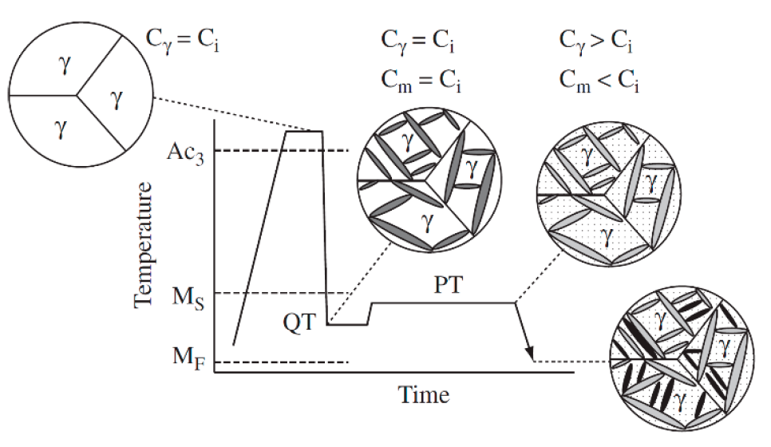
\includegraphics[width=0.75\textwidth]{Image/Q&P.png}
    \caption{Quenching and Partitioning process}
    \captionsetup{justification=centering,margin=2cm}
    \label{fig:QPprocess}
\end{figure}

%
Steel going through these two process contain 5 different phases: 

\begin{itemize}
    
    \item Ferrite is an alpha steel phase, meaning that it has the crystal structure of Body Centered Cubic (BCC). Ferrite is soft and ductile compare to martensite, which help with formability.
    
    \item Retained metastable austenite (RA) is a gamma steel phase, having Face Centered Cubic (FCC) crystal structure. Austenite is stable in high temperature (over 912 Celsius degree) and in room temperature, most of austenite convert to other phases. Austenite is soft and ductile compare to the other iron phases.
    
    \item Fresh Martensite is an alpha steel phase (BCC) created from the quenching process. Because of rapid cooling, the microstructure stop carbon from diffusing, creating a hard and compressed brittle structure.
    % Note for Ben secondary martensite? ask Zinan
    
    \item Tempered Martensite is an alpha steel phase (BCC) created from Fresh Martensite after the partitioning process. By heating martensite and slow cooling, relieving internal stress, martensite hardness and strength is slightly reduce while the microstructure stability and material ductility is significantly increased.
    
    \item Bainite is an alpha steel phase (BCC) created during the phase change of austenite. Bainite consists thin needle-like ferrite plate intercept with fine particle of cementite. 

\end{itemize}
This part is not completed.
\\
%picture
%Note: picture
\subsection{Target Material}
 In this study, the target material for analysis is QP1000 steel. QP1000 is a third generation advance high strength steel (AHSS).  The chemical compositing of the material is shown in Table \ref{chemcomp} \cite{QPprop}.

\begin{table}[h]
    \centering
    \captionsetup{justification=centering,margin=2cm}
    \caption{Chemical composition of QP1000, \% by mass}
    \begin{tabular}{| c | c | c | c | c | c | c | c |}
         \hline
         C & Si & Mn & Al & Cr & Co & Mo+Ni+Cu & P+S+Nb \\
         \hline
          0.15 & 1.67 & 2.42 & 0.074 & 0.02 & 0.026 & <0.01 & <0.006\\
         \hline
         
    \end{tabular}
    \label{chemcomp}
\end{table}

%mechanical properties
 The engineering stress-strain curve and true stress-strain curve of the material is present in Figure \ref{fig:Estressstrain}, \ref{fig:truess}.
 \begin{figure}
     \centering
     \captionsetup{justification=centering,margin=1cm}
     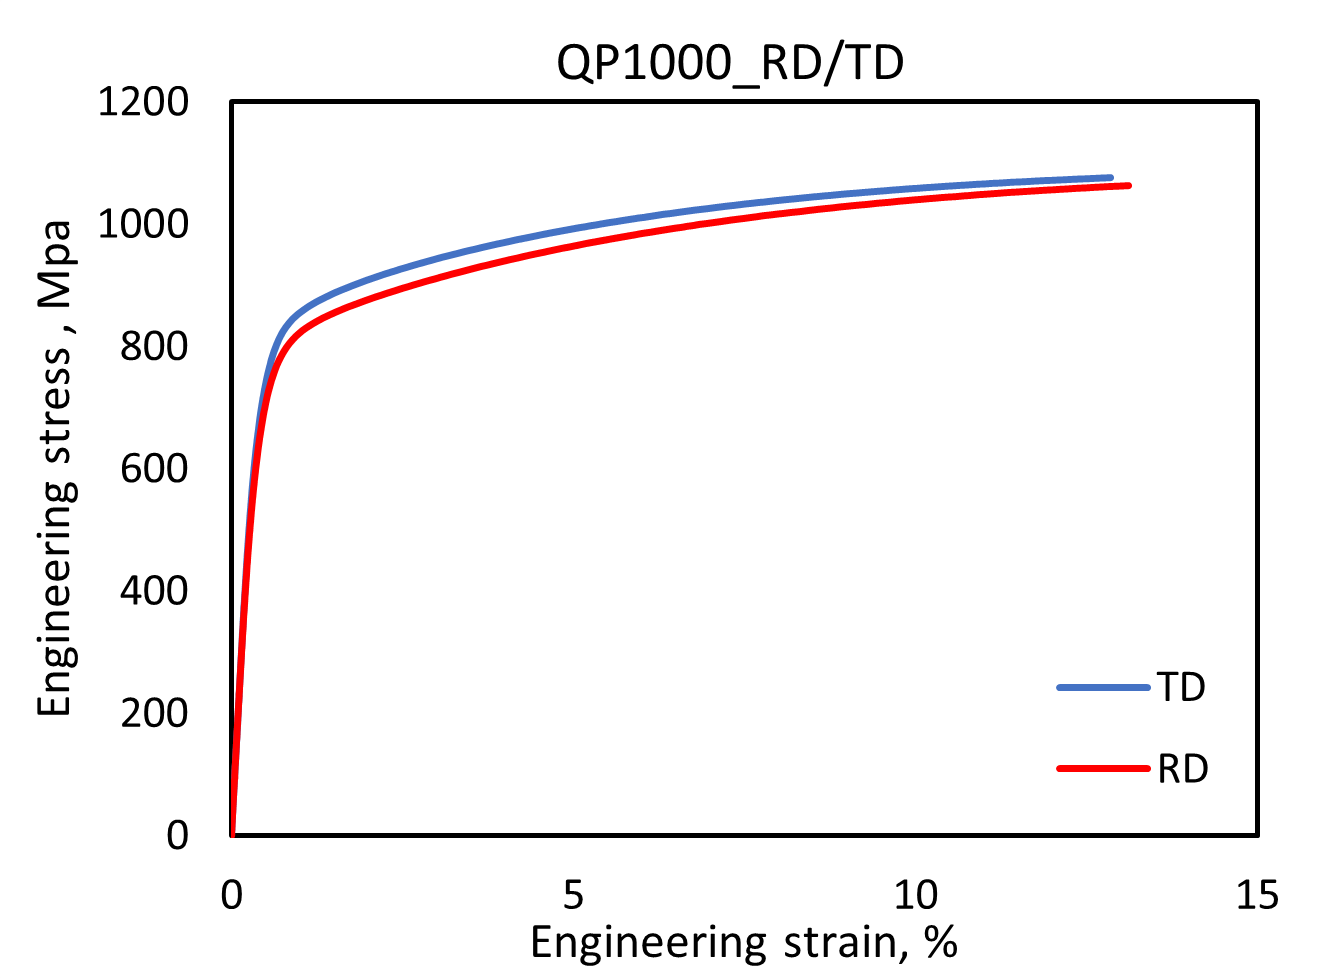
\includegraphics[width=0.8\linewidth]{Image/EngSSQP1000.png}
     \caption{QP1000 Engineering Stress-Strain Curve in RD and TD}
     \label{fig:Estressstrain}
 \end{figure}
 \begin{figure}
     \centering
     \captionsetup{justification=centering,margin=1cm}
     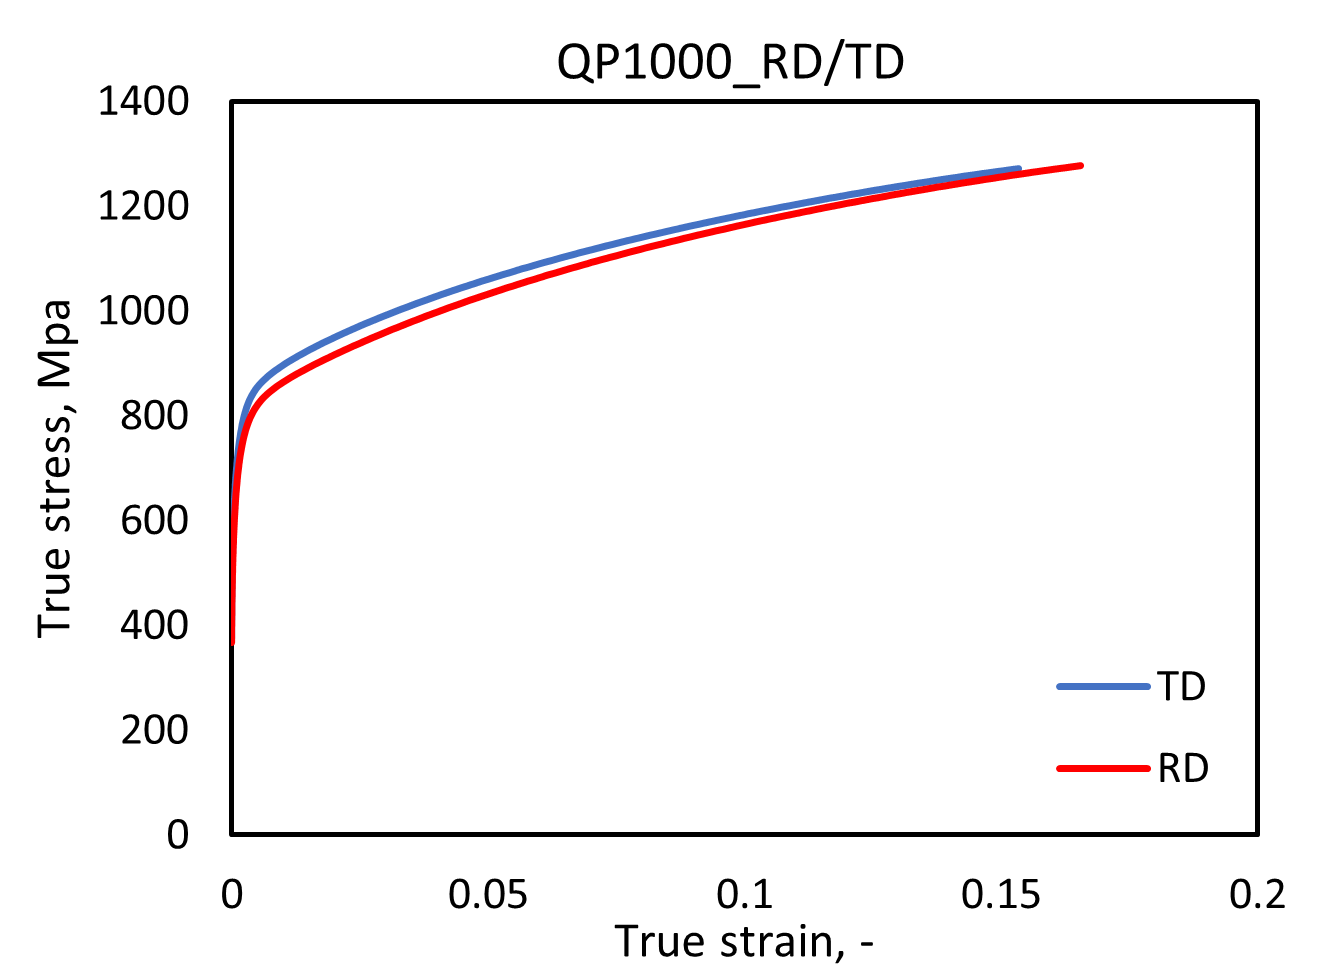
\includegraphics[width=0.8\linewidth]{Image/TrueSSQP1000.png}
     \caption{QP1000 True Stress-Strain Curve in RD and TD}
     \label{fig:truess}
 \end{figure}
 
 The mechanical properties of QP1000 steel is summarized in Table \ref{mechprop}. \cite{QPprop}.

\begin{table}[h]
    \centering
    \captionsetup{justification=centering,margin=2cm}
    \caption{Chemical composition of QP1000, \% by mass}
    \begin{tabular}{| c | c | c | c | c | }
         \hline
          YS, MPa  &  UTS, MPa  &  UE, \%  &  TE, \%  &  R-value at UE, -  \\
         \hline
        752.2 & 1090.20 & 18.09 & 23.57 & 0.75 \\
         \hline
         
    \end{tabular}
    \label{mechprop}
\end{table}





%%  METHODOLOGY  -------------------------------------------

\chapter{Methodology}
In this part, we propose an automatic pipeline for generating RVEs for Q\&P980 steel with high accuracy. First, a general pipeline for generating general RVE and post-evaluating is discussed. The pipeline is then extended to Q\&P980 steel by including phase segmentation for independent phase generation, and finally an extra step is presented to evaluate the spatial phase distribution of the generated multi-phase RVEs.

\section{Single-phase RVE generation and evaluation}
An existing pipeline for automatically generating and evaluating \textit{single-phase RVEs} is presented. Here, our main focus will be on the structures of the pipelines, possible computational optimizations, and the inclusion of the distribution curves of the material.

Given a known single-phase EBSD data, a pipeline for generating RVEs is given in Figure \ref{fig:generate}. The first step of the generation process is to extract the statistical data of the material's features from the EBSD. We will divide this into two parallel branches: the first one analyzes the grains' size and shape distribution of the material, and the second one extracts the ODF data from the EBSD. In the first branch, the grains are first fitted into equivalent ellipses: the corresponding ellipse has the same area as the grain's area. These ellipses have two important characteristics: their equivalent diameters (Figure \ref{fig:grainfit}) which tell us the size of the grains, and their aspect ratios which tell us the shape of the grains (values near 0 being extremely elongated and values near 1 being more equiaxed). 
\begin{figure}[h!]
    \captionsetup{justification=centering,margin=1cm}
    \centering
    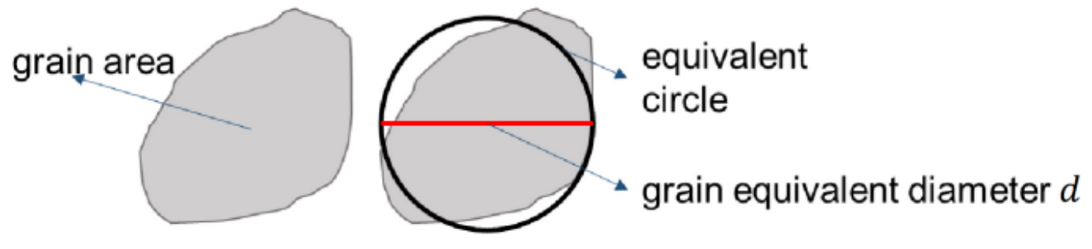
\includegraphics[width=0.75\textwidth]{Image/grainfit.png}
    \caption{RVE automatic generation pipeline.}
    \label{fig:grainfit}
\end{figure}
The grains' equivalent diameters $d$ are then fitted into a \textit{log-normal distribution} with the formula:
\begin{equation}
f(d; \mu, \sigma)dy = \frac{1}{d\sigma \sqrt{2\pi}}e^{-\frac{(\ln d - \mu)^2}{2\sigma^2}}dy
\end{equation}
By using maximum likelihood estimation, we can find the corresponding value $\mu$ and $\sigma$ for the distribution of our empirical equivalent diameters data. The average size (diameter) can be calculated from the distribution as:
\begin{equation}
\bar{d} = e^{\left(\mu+\frac{\sigma^2}{2}\right)}
\end{equation}
Similarly, we also fit the aspect ratio data $x$ using a \textit{beta distribution} with the formula:
\begin{equation}
f(x; \alpha, \beta)dy = \frac{\Gamma(\alpha + \beta)}{\Gamma(\alpha)\Gamma(\beta)}x^{\alpha - 1}(1 - x)^{\beta - 1}dy
\end{equation}
and get the distribution parameters $\alpha$ and $\beta$ using maximum likelihood estimation, and the empirical average aspect ratio can be calculated as:
\begin{equation}
\Bar{x} = \frac{\alpha}{\alpha + \beta} 
\end{equation}
The fitting of equivalent ellipses and estimation of distribution curves can be done in MTEX - an open-source toolbox for analyzing and modeling crystallographic textures by means of EBSDs. In the second branch, we utilize DREAM3D - a collection of data analysis tools for materials science research - to build a separate pipeline and extract the ODF data into a separate file. An existing pipeline \textit{Export StatsGenerator ODF Angle File} would export a file with Euler angles data ($\varphi_1$, $\phi$, $\varphi_2$), weight $w$, and $\sigma$, and this file will be used as an input for the ODF data of the RVE generation.
\begin{figure}[h!]
    \captionsetup{justification=centering,margin=1cm}
    \centering
    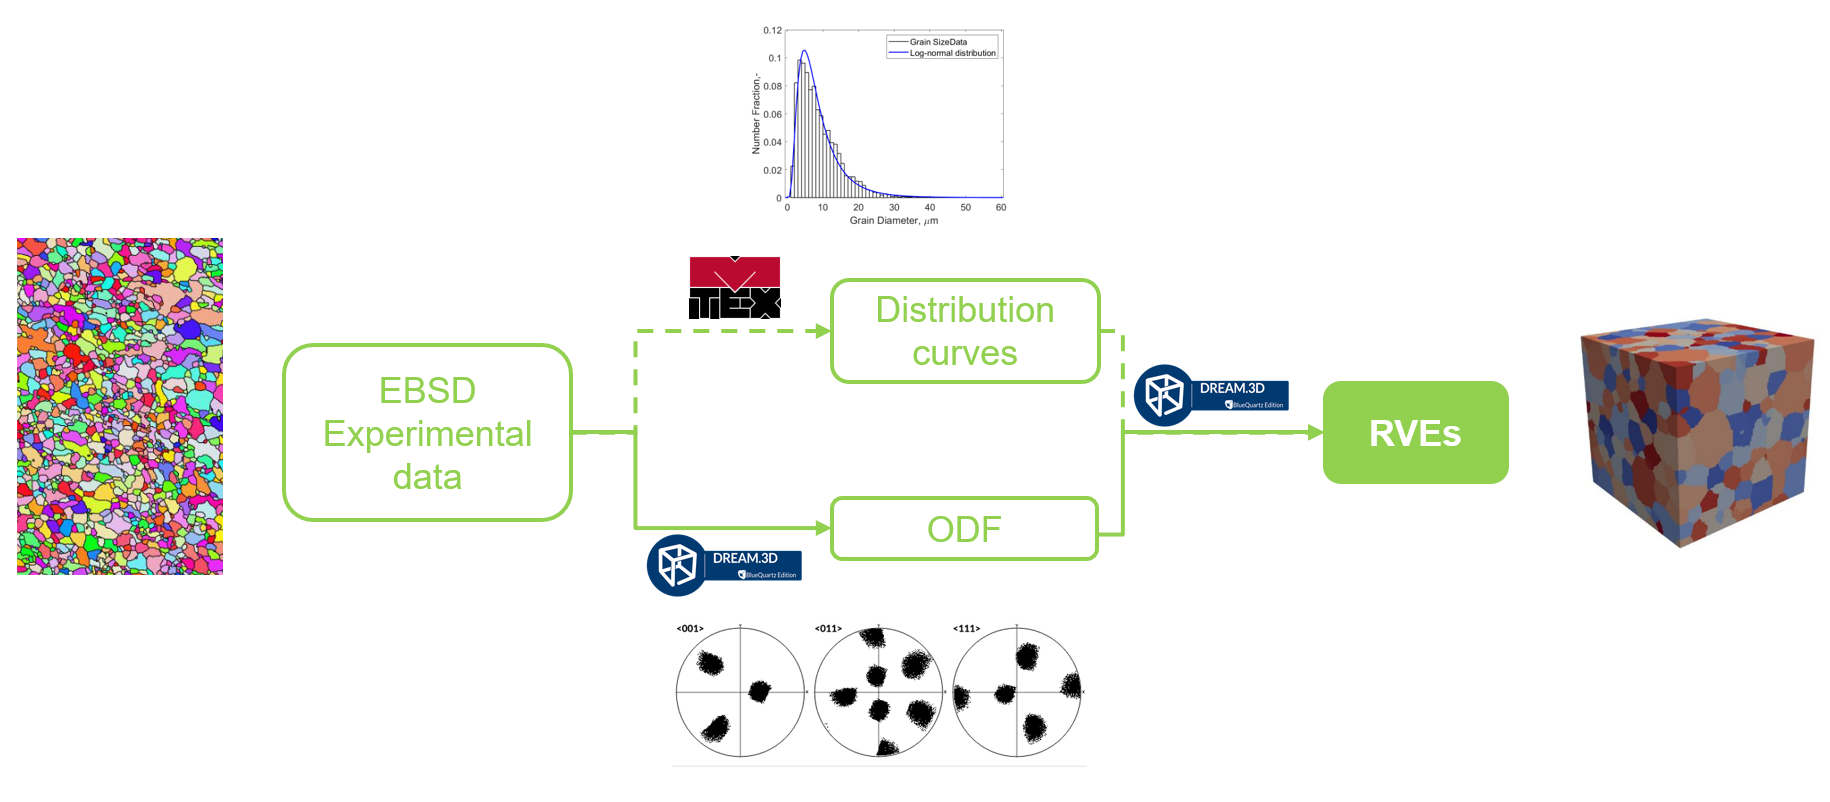
\includegraphics[width=1.0\textwidth]{Image/rve pipeline.png}
    \caption{RVE automatic generation pipeline.}
    \label{fig:generate}
\end{figure}

The next step in our generation process is building a pipeline for RVE generation on DREAM3D. The pipeline includes the following filters:
\begin{itemize}
    \item StatsGenerator: this filter takes in $\mu$ and $\sigma$ for log-normal size distribution, $\alpha$ and $\beta$ for beta shape distribution, and the ODF file produced earlier as input for RVE's ODF.
    \item Initialize Synthetic Volume: creates an empty volume as a base for inserting features to create a synthetic microstructure. Here, the dimension of our RVE will be 100$\times$100$\times$100 to capture both small and large grains, and the resolution will be set to 5$\times$5$\times$5. %hallo
    \item Establish Shape Types: here we assign the \textit{ellipsoid} shape type to each ensemble of a synthetic structure.
    \item Pack Primary Phases: place precipitate features with the sizes, shapes, physical orientations and locations corresponding to the goal statistics.
    \item Find Feature Neighbors: determines, for each feature, the number of other Features that are in contact with it.
    \item Match Crystallography: match a defined orientation distribution function (ODF) to a set of features using a "switch or swap" approach.
    \item Generate IPF Colors: generate \textit{inverse pole figure (IPF)} colors for our cubic crystal structures.
    \item Write DREAM.3D Data File: write the contents of the current data structure to an HDF5 based file with the file extension .dream3d. This file will be used for future access to the RVE.
    \item Export Feature Data as CSV File: writes the data associated with each Feature to a file in CSV format. This file will be used for RVE evaluation process.
    \item Export Los Alamos FFT File: writes out cell data from an image geometry to a TXT file. This file will be used for RVE evaluation process.
\end{itemize}
This part is not completed.
----------------------------------

% ------------------ Evaluation
An important step in RVE generation is the post-evaluation process, where the generated RVE is compared to the original material on several characteristics: the smaller the difference, the more representative of the material our RVE is. This is not a simple task however, since comparing a 3D structure with a 2D EBSD scan requires some extra preprocessing, and the choices of features for evaluation are are also restricted. We will first discuss an existing process for evaluating RVEs regarding their size and shape distribution, and from here we extend the process by including misorientation into the evaluation.

An existing pipeline for evaluating RVEs is given in Figure \ref{fig:evaluate}.

\begin{figure}[h!]
    \captionsetup{justification=centering,margin=1cm}
    \centering
    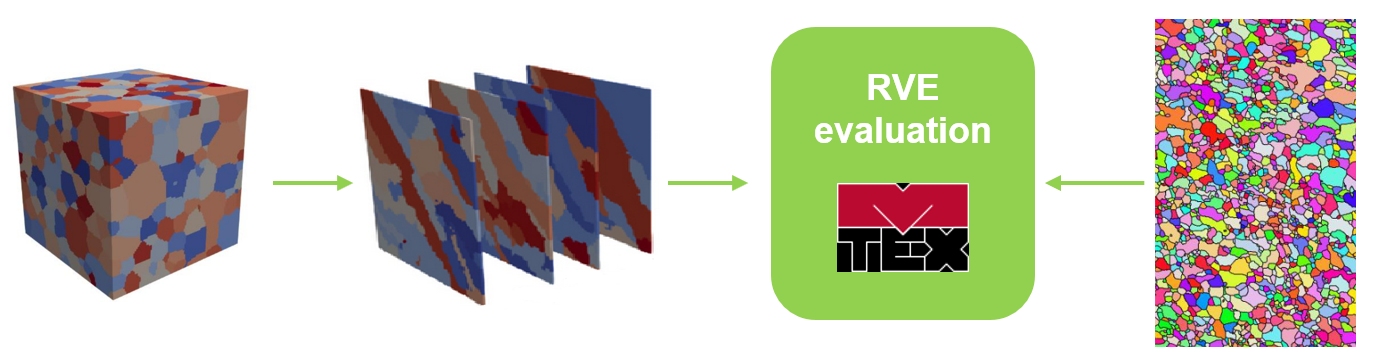
\includegraphics[width=1.0\textwidth]{Image/evaluation.png}
    \caption{RVE automatic evaluation pipeline: an extra step includes slicing the generated RVE along z-axis \cite{Azhari2022}.}
    \label{fig:evaluate}
\end{figure}

This part is not finished yet.

\section{Pipeline extension to Q\&P steel generation}
The introduction of the pipeline to Q\&P steel is not straightforward, since Q\&P steel is a multi-phase material: different distributions are required for different phases, and the distribution of phases in the microstructure is also of great importance. Therefore, a separate process for accurately identifying different phases (namely ferrite, austenite, fresh martensite, tempered martensite, and bainite) inside Q\&P steel is discussed, and a new method for evaluating the spatial distribution of phases in the microstructure is proposed.
\\
\subsection{Phase segmentation methods for Q\&P steel}
%This part is in process.
In order to accurately represent the steel microstructure, the model need to contain different phases inside the material. Generating different phases in RVE require the microstructure information from different phases. Hence, phases identification and segmentation is needed for generating the RVE. 

The current phase segmentation criteria is presented in Table \ref{segmentation}. 

\begin{table}[h]
    \centering
    \captionsetup{justification=centering,margin=2cm}
    \caption{Segmentation Criteria for Different Steel Phases}
    \begin{tabular}{| c | c | c | c | c | c | }
         \hline
          Phases  &  CS  &  IQ  &  GOS  &  KAM & Grain size  \\
         \hline
        Austenite & FCC & - & - & - & Small\\
         \hline
         Ferrite & BCC & High & Low & Low & Large \\
         \hline
         Fresh Martensite & BCC & Low & Low & Low & Small\\
         \hline
         Tempered Martensite & BCC & High & High & High & Large \\
         \hline
         Bainite & BCC & Medium/High & High & High & Small \\
         \hline
         
    \end{tabular}
    \label{segmentation}
\end{table}

Having different properties, different phases of steel can be separated. Austenite can be detected as it have a FCC crystal structure, which is different from the other phases' BCC crystal structure. Because of the rough surface, fresh martensite can be identify having a lower image quality (IQ). Another variable can be consider in order to divide the phases are also grain orientation spread (GOS), detecting tempered martensite and bainite. Finally, because of the particular shape, bainite can be identify within the phases.

%Need to rewrite. Do you think we should state which criteria and then the corresponding phase detected.
% Second note: can make both of these into a figure using subfigure
\begin{figure}
    \centering
    \captionsetup{justification=centering,margin=1cm}
    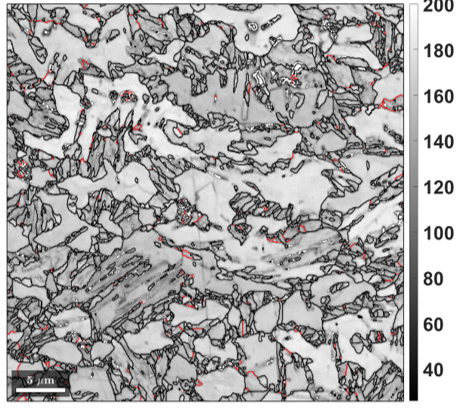
\includegraphics[width=0.6\linewidth]{Image/IQ QP980.png}
    \caption{Image Quality map from QP980}
    \label{fig:enter-label}
\end{figure}
\begin{figure}
    \centering
    \captionsetup{justification=centering,margin=1cm}
    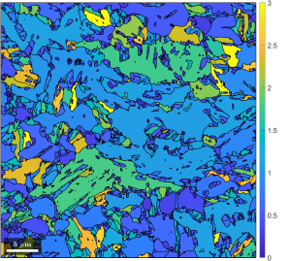
\includegraphics[width=0.6\linewidth]{Image/GOS QP980.png}
    \caption{Grain Orientation Spread map from QP980}
    \label{fig:enter-label}
\end{figure}


\subsection{Multi-phase spatial distribution evaluation}

So far, we have discussed on how to evaluate the quality of our generated RVEs based on the size, shape, and \textbf{misorientation} distribution of each individual phase contained in Q\&P980 steel. However, another important characteristic of multiphasic materials that we have not considered so far is the spatial distribution of the phases in the material. In other words, we want to know how the phases are distributed inside the material, which is different from the characteristics of the grains of each phase. For this purpose, we propose one efficient and effectively accurate method called \textit{2-point spatial correlations} (also called 2-point statistics). The idea of 2-point statistics is as following: given 2 phases $l$ and $l'$, the 2-point statistics equation gives us the probability that a vector of random magnitude and direction in the microstructure will have one end at $l$ and the other end at $l'$ \cite{Yucel2020}. The equation of 2-point statistics is given below:
\begin{equation}
f(\vec{r} \vert l, l') = \frac{1}{S}\sum_{s} m(s, l)m(s+\vec{r}, l')
\end{equation}
Here, $f(\vec{r} \vert l, l')$ is the conditional probability of finding the phase $l$ and $l'$ at a distance and orientation away from each other given the vector $\vec{r}$, both $m(s, l)$ and $m(s+\vec{r}, l')$ are probability density functions of finding phase $l$ at location $s$ ($s$ is a specific spatial bin in the microstructure) and phase $l'$ at location $s+\vec{r}$, and $S$ is the total number of spatial bins in the microstructure. It is clear that 2-point statistics encodes both the fractions of phases and the distribution of the phases inside the microstructure. The method is referred to as \textit{autocorrelation} if the two phases are the same $l = l'$, and \textit{cross-correlation} if $l$ and $l'$ are two different phases.

In this project, we will evaluate the spatial distribution of multi-phase Q\&P steel for 5 phases: ferrite, austenite, fresh martensite, tempered martensite, and bainite. The method of correlation would be autocorrelation to optimize both the representativeness of the results and the computational resources of the pipeline (cross-checking all 10 combinations of correlation pairs would consume double the time and memory resources), and the computation is ultilized using the open-source library PyMKS.


\chapter{Result}
This part is in process hehe.
\section{Single phase analysis and evaluation}
The grains data collected using the AISI439 Stainless Steel EBSD analysis is shown in Table \ref{singlephase}. Moreover, the texture file (ODF) of the material was generated and collected from Dream3D.

\begin{table}[h]

\begin{tabular}{|ll|ll|}
\hline
\multicolumn{2}{|l|}{Grain size distribution}    & \multicolumn{2}{l|}{Grain Shape Distribution}    \\ \hline
\multicolumn{1}{|l|}{$ \mu$ } &  $ \sigma$   & \multicolumn{1}{l|}{$ \alpha $  } & $ \beta$  \\ \hline
\multicolumn{1}{|l|}{ 3.5503} &  0.5996   & \multicolumn{1}{l|}{3.1206} & 1.3618  \\ \hline
\end{tabular}
\centering
\captionsetup{justification=centering,margin=2cm}
\caption{Grain data from AISI439}
\label{singlephase}
\end{table}


The RVEs was generated using different configuration consist of the resolution and dimension. The configuration was chosen such that there would be at least 1000 grain generated. These RVEs are then evaluated and compare to each other. The grain number and mean error are presented in Table \ref{error_table} 

\begin{table}[h]
    \centering
    \captionsetup{justification=centering,margin=2cm}
    \caption{Error from the original file, \%. The Italic* number RVEs does not satisfy the amount of grain}
    \begin{tabular}{| c | c | c | c | c | c | }
         \hline
          Resolution  &  4  &  4.5  &  5  &  5.5 & 6  \\
         \hline
         80 x 80 x 80 & \textit{1.16*}  & \textit{1.68*} & \textit{3.15*} & \textit{1.50*} & 4.28\\
         \hline
         100 x 100 x 100 & \textit{4.26*} & \textit{3.43*}& 4.27 & \textbf{2.72} & 3.40 \\
         \hline
         120 x 120 x 120 & 3.36 & 2.95 & 4.04 & 2.88 & 2.87 \\
         \hline
    \end{tabular}
    \label{error_table}
\end{table}

According to the result, we find that the best configuration is dimension 100x100x100 and resolution 5.5. The data was input to the pipeline in CSC which would utilize dream 3D to generate the RVEs. In total 50 RVEs of this configuration was generated and evaluated for the project. The optimal RVE has the error of 1.906. The distribution of error in the different RVEs is shown in Figure.


\section{Material Microstructure Analysis}
% The microstructure of the material is provided in an EBSD file. Its properties are characterized with regards to RVE generation: 
% Do you think we should use section on this like a) b) ect
\begin{itemize}
   \item Grain size 
    
   \item Grain aspect
    
   \item Orientation

   \item Misorientation

   \item Tilt angle
    
\end{itemize}


\section{RVE generation result}


%\section{RVE development result}

\chapter{Discussion}
This part is in process.

\chapter{Self-evaluation}
This part is in process.
%My lawyer has advise not to do any joke here
\renewcommand{\bibname}{Reference}
\bibliographystyle{ieeetr} % We choose the "ieee" reference style
\bibliography{refs}
%%  LIITTEET  ------------------------------------------

%\appendix

%chapter{Ut purus elit}



\end{document}
